\documentclass[letterpaper, 10 pt, conference]{ieeeconf}
\usepackage{graphicx}
\overrideIEEEmargins

\usepackage[utf8]{inputenc}
\usepackage[T1]{fontenc}
\usepackage{amsmath}
\usepackage{amssymb}
\usepackage{booktabs}
\usepackage{array}
\usepackage{etoolbox}
\graphicspath{{figs/}}
\makeatletter
\def\fnum@table{TABLA~\thetable}
\patchcmd{\thebibliography}{\section*{References}}{\section*{Referencias}}{}{}
\makeatother

\title{\LARGE \bf
Clasificación de sentimientos de reseñas de IMDb con redes neuronales recurrentes, embeddings preentrenados y ensambles
}

\author{Miguel Muñoz, David Cardenas y Mario Celis}

\begin{document}

\maketitle
\thispagestyle{empty}
\pagestyle{empty}

%%%%%%%%%%%%%%%%%%%%%%%%%%%%%%%%%%%%%%%%%%%%%%%%%%%%%%%%%%%%%%%%%%%%%%%%%%%%%%%%
\section{Introducción}

Clasificar automáticamente la polaridad de reseñas de películas permite resumir la recepción de una obra y alimentar sistemas de recomendación. El problema es difícil porque el sentimiento depende del contexto: negaciones (\textit{not bad at all}), contrastes e ironía (\textit{so bad it's good}) invierten el significado de las palabras aisladas.

Las redes recurrentes con compuertas, LSTM~\cite{c1} y GRU~\cite{c2}, leen el texto en orden y mantienen un estado que resume el contexto. Necesitan representar las palabras como vectores densos, que Word2Vec~\cite{c3} y GloVe~\cite{c4} aprenden sin supervisión. Aun así, en IMDb los modelos lineales de bolsa de bigramas son una línea base muy fuerte~\cite{c5,c6}, porque la polaridad suele expresarse con frases cortas.

El objetivo es clasificar reseñas de IMDb con una RNN y reportar precision, recall y F1 en prueba. A partir de una versión previa (BiGRU con Word2Vec, F1 $=0{,}9119$), este trabajo: (i) compara Word2Vec entrenado en el dominio con GloVe preentrenado; (ii) evalúa congelar el embedding para controlar el sobreajuste; (iii) ajusta umbral, temperatura y ensambles en validación, y (iv) reporta todo con 3 semillas frente a una línea base TF-IDF.

\section{Metodología}

\textbf{Datos.} Se usó el conjunto \textit{IMDB Movie Ratings Sentiment Analysis} de Kaggle: 40\,000 reseñas en inglés etiquetadas como negativa (0) o positiva (1), con clases balanceadas. Se eliminó el HTML, se pasó a minúsculas y se tokenizó conservando contracciones (\textit{didn't}) y los signos \texttt{!}/\texttt{?}, sin quitar \textit{stopwords}, porque \textit{not} o \textit{but} deciden la polaridad. Para evitar fuga de datos se eliminaron 280 duplicados antes de partir. La partición es estratificada 70/15/15: 27\,804 / 5\,958 / 5\,958 reseñas. El vocabulario (20\,002 términos con frecuencia $\geq 2$) se construye solo con entrenamiento. Cada reseña se trunca a 200 tokens ($\frac{1}{4}$ inicial y $\frac{3}{4}$ finales), lo que deja completo el 58\,\% de las de entrenamiento.

\textbf{Embeddings} (dimensión 100). Se compararon dos: Word2Vec \textit{skip-gram}~\cite{c3} (ventana 5), entrenado solo con entrenamiento, y GloVe 6B~\cite{c4} (Wikipedia + Gigaword). En GloVe, cada contracción recibe el promedio de sus partes (\textit{did}, \textit{n't}), lo que sube su cobertura del 96,6\,\% al 99,6\,\%.

\textbf{Arquitectura.} Embedding $20\,002\times100$ (entrenable o congelado) $\rightarrow$ dropout 0,3~\cite{c7} $\rightarrow$ GRU bidireccional~\cite{c8} de 1 capa con 64 unidades por dirección $\rightarrow$ promedio y máximo de las salidas (256) $\rightarrow$ dropout 0,3 $\rightarrow$ capa densa con sigmoide, que da $P(\text{positiva})$. Las compuertas mitigan el desvanecimiento del gradiente~\cite{c9}, y el máximo retiene expresiones fuertes aunque aparezcan a mitad del texto. Fue la mejor en validación en la versión previa. Tiene 2,06\,M de parámetros, el 97\,\% en el embedding; al congelarlo quedan 64\,k entrenables.

\textbf{Entrenamiento.} Entropía cruzada binaria con Adam~\cite{c10} (tasa de aprendizaje $10^{-3}$, lotes de 128) y \textit{clipping} de norma 1~\cite{c11}. La tasa se reduce a la mitad si la F1 de validación se estanca. Máximo 10 épocas con \textit{early stopping} (paciencia 3) sobre la F1 de validación. Semillas 42, 7 y 123.

\textbf{Postproceso.} Con las predicciones de \emph{validación} se eligen: el umbral que maximiza la F1; la temperatura $T$ que minimiza la \textit{log-loss}~\cite{c12}; el promedio de semillas, y el peso $w$ de $w\,P_{\text{RNN}}+(1-w)\,P_{\text{TF-IDF}}$. La línea base es TF-IDF de 1-2 gramas sobre la reseña completa con regresión logística~\cite{c6}. El conjunto de prueba solo se usa para reportar.

\textbf{Métricas.} Precision, recall y F1 de la clase positiva (las que pide el enunciado; balancean falsos positivos y negativos), accuracy, ROC-AUC (independiente del umbral) y el error de calibración esperado (ECE). Se calcula un IC 95\,\% por \textit{bootstrap} (1\,000 remuestreos). El código está en \texttt{01\_solucion\_rnn\_imdb\_2.ipynb}.

\begin{figure*}[t]
\centering
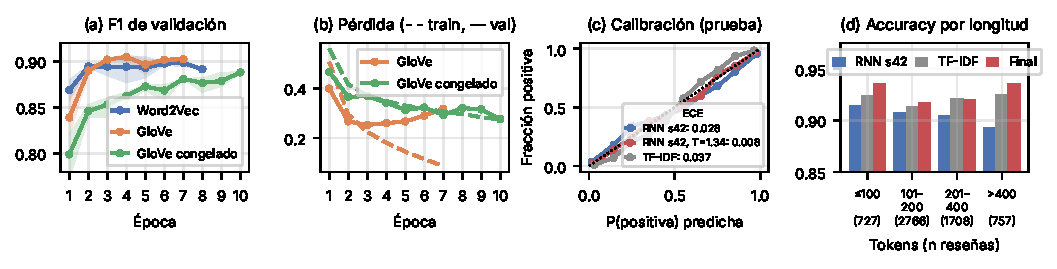
\includegraphics[width=\textwidth]{fig1_entrenamiento_calibracion_longitud.pdf}
\caption{(a) F1 de validación por época (media y rango de 3 semillas). (b) Pérdida media de entrenamiento (discontinua) y validación (continua), GloVe entrenable y congelado. (c) Diagrama de confiabilidad en prueba de la RNN (semilla 42) antes y después de la calibración, y de TF-IDF. (d) Accuracy en prueba por longitud de la reseña.}
\label{fig:curvas}
\end{figure*}

\section{Resultados}

\textbf{Cuantitativos.} La Tabla~\ref{tab:res} resume los resultados en prueba. Word2Vec y GloVe empatan ($0{,}9044\pm0{,}0010$ frente a $0{,}9040\pm0{,}0028$). Se eligió GloVe por su mayor F1 de validación ($0{,}9057$ frente a $0{,}9036$). Congelar el embedding baja la F1 a $0{,}8907$. El congelado mejora lentamente hasta la época 10 (Fig.~\ref{fig:curvas}a), mientras el entrenable sobreajusta desde la época 3: su pérdida de validación sube y la de entrenamiento cae (Fig.~\ref{fig:curvas}b).

\begin{table}[t]
\centering
\caption{Resultados en prueba (5\,958 reseñas); (3s): media $\pm$ desv. est. de 3 semillas. 200 tokens salvo v1.}
\label{tab:res}
\setlength{\tabcolsep}{2.4pt}
\footnotesize
\begin{tabular}{@{}lccccc@{}}
\toprule
\textbf{Modelo} & \textbf{Acc.} & \textbf{P} & \textbf{R} & \textbf{F1} & \textbf{AUC} \\
\midrule
TF-IDF + reg. logística & 0,918 & 0,916 & 0,921 & 0,9187 & 0,972 \\
v1: BiGRU W2V, 400 tok. (3s) & 0,911 & 0,902 & 0,923 & 0,9119$\pm$0,0034 & 0,969 \\
\midrule
BiGRU Word2Vec (3s) & 0,902 & 0,889 & 0,920 & 0,9044$\pm$0,0010 & 0,963 \\
BiGRU GloVe (3s) & 0,903 & 0,895 & 0,913 & 0,9040$\pm$0,0028 & 0,964 \\
BiGRU GloVe congelado (3s) & 0,889 & 0,879 & 0,904 & 0,8907$\pm$0,0014 & 0,958 \\
GloVe + umbral (3s) & 0,903 & 0,895 & 0,914 & 0,9044$\pm$0,0029 & 0,964 \\
GloVe, ens. 3 sem. + umbral & 0,903 & 0,889 & 0,922 & 0,9054 & 0,965 \\
GloVe + TF-IDF + umbral (3s) & 0,921 & 0,916 & 0,927 & 0,9213$\pm$0,0015 & 0,974 \\
\textbf{Ens. 3 sem. + TF-IDF + umbral} & \textbf{0,923} & \textbf{0,920} & \textbf{0,927} & \textbf{0,9231} & \textbf{0,974} \\
\bottomrule
\end{tabular}
\end{table}

El umbral ajustado (entre 0,47 y 0,53) cambia la F1 en solo $+0{,}0004$. La temperatura ($T=1{,}14$ a $1{,}35$) baja el ECE de 0,024 a 0,009 sin cambiar las predicciones (Fig.~\ref{fig:curvas}c). Ensamblar con TF-IDF ($w=0{,}4$ a $0{,}5$) y umbral ajustado sube la F1 a $0{,}9213\pm0{,}0015$. El sistema final, elegido por F1 de validación, combina el promedio de 3 semillas con TF-IDF: obtiene F1 $=0{,}9231$ (IC 95\,\%: 0,9160 a 0,9299), con 242 falsos positivos y 219 falsos negativos (Fig.~\ref{fig:cual}b). Frente a la línea base la diferencia es $+0{,}0044$, con IC 95\,\% de $-0{,}0012$ a $+0{,}0100$. En las reseñas de más de 400 tokens, la RNN sola acierta 0,893, TF-IDF 0,925 y el sistema final 0,935 (Fig.~\ref{fig:curvas}d).

\textbf{Cualitativos.} La Tabla~\ref{tab:cual} muestra reseñas de prueba con su etiqueta real y la probabilidad de cada modelo. En la Fig.~\ref{fig:cual}a, la RNN y TF-IDF discrepan en 469 reseñas (7,9\,\%), justo la zona que resuelve la frontera del ensamble. Frente a la RNN (semilla 42), el sistema final corrige 157 errores, introduce 55 y baja los errores con confianza $>0{,}9$ de 177 a 54.

\begin{figure}[t]
\centering
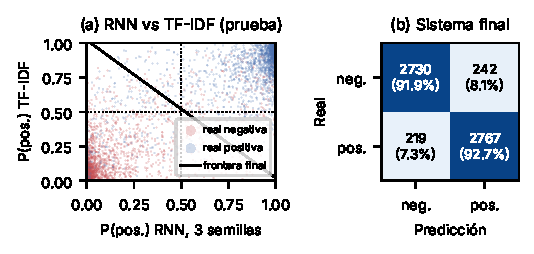
\includegraphics[width=\columnwidth]{fig2_rnn_vs_tfidf_confusion.pdf}
\caption{(a) $P(\text{positiva})$ del ensamble de 3 semillas de la RNN frente a TF-IDF en prueba, coloreada por la etiqueta real. Las líneas punteadas son el umbral 0,5 de cada modelo y la continua es la frontera del sistema final. (b) Matriz de confusión del sistema final.}
\label{fig:cual}
\end{figure}

\begin{table}[t]
\centering
\caption{Ejemplos de prueba: etiqueta real y $P(\text{positiva})$ de la RNN (semilla 42), de TF-IDF y del sistema final.}
\label{tab:cual}
\setlength{\tabcolsep}{2.2pt}
\scriptsize
\begin{tabular}{@{}>{\raggedright\arraybackslash}p{4.45cm}cccc@{}}
\toprule
\textbf{Reseña (inicio)} & \textbf{Real} & \textbf{RNN} & \textbf{TF-IDF} & \textbf{Final} \\
\midrule
\textit{certainly one of the finest movies...} & + & 1,00 & 1,00 & 1,00 \\
\textit{this is the worst movie i have ever...} & $-$ & 0,00 & 0,00 & 0,00 \\
\textit{this movie was pure genius john waters...} & $-$ & 1,00 & 1,00 & 1,00 \\
\textit{...makes a bad movie worth watching...} & + & 0,00 & 0,00 & 0,00 \\
\textit{far too few mainstream films...} (690 tok.) & + & 0,19 & 0,93 & 0,65 \\
\textit{as a big fan of the original film...} & $-$ & 0,91 & 0,05 & 0,45 \\
\bottomrule
\end{tabular}
\end{table}

\section{Discusión}

\textbf{Embeddings.} Inicializar con vectores preentrenados importa más que su fuente. En la versión previa, pasar de embeddings aleatorios a Word2Vec sumó entre 2 y 3 puntos de F1; aquí GloVe y Word2Vec empatan. Al ser entrenable, el embedding (2\,M parámetros) se adapta a la tarea y borra la diferencia de partida: GloVe empieza peor y alcanza a Word2Vec en la época 3 (Fig.~\ref{fig:curvas}a). Además, GloVe codifica co-ocurrencia general y no polaridad (entre los vecinos de \textit{boring} está \textit{funny}), una limitación ya descrita para el análisis de sentimiento~\cite{c5}.

\textbf{Capacidad y sesgo-varianza.} Con 2\,M de parámetros y 28\,k reseñas, el modelo entrenable memoriza desde la época 3, y es el \textit{early stopping} el que controla su varianza (brecha de accuracy entre entrenamiento y validación de 0,020). Congelar el embedding cambia varianza por sesgo: la brecha cae a $-0{,}003$, pero el modelo subajusta (1,3 puntos menos de F1), porque 64\,k parámetros no bastan para separar palabras que GloVe deja cerca pese a tener polaridad opuesta.

\textbf{Calibración.} $T>1$ en todas las semillas indica que la red es sobreconfiada, algo típico de redes entrenadas con entropía cruzada~\cite{c12}. El umbral óptimo quedó cerca de 0,5 porque los errores ya están equilibrados, a diferencia de la versión previa (375 falsos positivos frente a 175 falsos negativos).

\textbf{Complementariedad.} El ensamble con TF-IDF es la mejora principal (+1,7 puntos sobre la RNN), porque los errores de los dos modelos están poco correlacionados: la RNN modela el orden pero lee solo 200 tokens, mientras TF-IDF ve la reseña completa sin orden~\cite{c6}. Promediarlos reduce la varianza; así se corrigen la reseña larga y la crítica del \textit{remake} de la Tabla~\ref{tab:cual}. La mejora frente a TF-IDF no es significativa, porque su IC incluye el cero.

\textbf{Limitaciones y mejoras.} Los errores más confiados, compartidos por todos los modelos, son ruido de etiquetado probable (\textit{pure genius} etiquetada como negativa) e ironía; fijan un techo al desempeño. La RNN con 200 tokens (0,904) queda por debajo de la v1 con 400 (0,912). Se proponen: (i) GloVe con 400 tokens más el ensamble; (ii) descongelar el embedding gradualmente, y (iii) leer las reseñas largas por segmentos o con atención.

\begin{thebibliography}{99}

\bibitem{c1} S. Hochreiter and J. Schmidhuber, ``Long short-term memory,'' \textit{Neural Comput.}, vol. 9, no. 8, pp. 1735--1780, 1997.
\bibitem{c2} K. Cho \textit{et al.}, ``Learning phrase representations using RNN encoder-decoder for statistical machine translation,'' in \textit{Proc. EMNLP}, 2014, pp. 1724--1734.
\bibitem{c3} T. Mikolov, K. Chen, G. Corrado, and J. Dean, ``Efficient estimation of word representations in vector space,'' arXiv:1301.3781, 2013.
\bibitem{c4} J. Pennington, R. Socher, and C. D. Manning, ``GloVe: Global vectors for word representation,'' in \textit{Proc. EMNLP}, 2014, pp. 1532--1543.
\bibitem{c5} A. L. Maas, R. E. Daly, P. T. Pham, D. Huang, A. Y. Ng, and C. Potts, ``Learning word vectors for sentiment analysis,'' in \textit{Proc. ACL-HLT}, 2011, pp. 142--150.
\bibitem{c6} S. Wang and C. D. Manning, ``Baselines and bigrams: Simple, good sentiment and topic classification,'' in \textit{Proc. ACL}, 2012, pp. 90--94.
\bibitem{c7} N. Srivastava, G. Hinton, A. Krizhevsky, I. Sutskever, and R. Salakhutdinov, ``Dropout: A simple way to prevent neural networks from overfitting,'' \textit{J. Mach. Learn. Res.}, vol. 15, pp. 1929--1958, 2014.
\bibitem{c8} M. Schuster and K. K. Paliwal, ``Bidirectional recurrent neural networks,'' \textit{IEEE Trans. Signal Process.}, vol. 45, no. 11, pp. 2673--2681, 1997.
\bibitem{c9} Y. Bengio, P. Simard, and P. Frasconi, ``Learning long-term dependencies with gradient descent is difficult,'' \textit{IEEE Trans. Neural Netw.}, vol. 5, no. 2, pp. 157--166, 1994.
\bibitem{c10} D. P. Kingma and J. Ba, ``Adam: A method for stochastic optimization,'' in \textit{Proc. ICLR}, 2015.
\bibitem{c11} R. Pascanu, T. Mikolov, and Y. Bengio, ``On the difficulty of training recurrent neural networks,'' in \textit{Proc. ICML}, 2013, pp. 1310--1318.
\bibitem{c12} C. Guo, G. Pleiss, Y. Sun, and K. Q. Weinberger, ``On calibration of modern neural networks,'' in \textit{Proc. ICML}, 2017, pp. 1321--1330.

\end{thebibliography}

\end{document}
